\chapter{Infraestrutura}
\minitoc
\clearpage

\section{Contextualización}

O desenvolvemento deste proxecto está contextualizado no \gls{CESGA}, o centro de cálculo, comunicacións de altas prestacións e servizos avanzados da Comunidade Científica Galega, do Sistema Académico Universitario e do Consello Superior de Investigacións Científicas (CSIC). Cómpre coñecer as singularidades que un centro \gls{HPC} posúe no tratamento con contedores, polo que a súa infraestrutura e a relación con esta tecnoloxía de virtualización serán explicadas polo miúdo neste capítulo.

\section{Finis Terrae II}
\label{recursosFT2}

Finis Terrae II é un sistema de computación xestionado polo \gls{CESGA} e integrado na Rede Española de Supercomputación, considerada unha Infraestrutura Científica e Técnica Singular (ICTS). Trátase dun \textit{cluster} Linux heteroxéneo, baseado en procesadores Intel Haswell e interconectado mediante rede InfiniBand cun rendemento pico de 328 TFlops e sostido en Linpack de 213 Tflops. Posúe unha rede de Interconexión de alto rendemento Mellanox InfiniBand FDR@56Gbps con topoloxía \textit{Fat-tree} e un sistema de ficheiros paralelo Lustre con 768TB de capacidade (750TB netos) e 20GB/s de lectura/escritura cun consumo total de 118Kw e rendemento pico de 328 TFlops (240 Tflops Linpack) \cite{FT2CESGA}. Unha representación de dita arquitectura pode ser apreciada nas figuras \ref{FT2_1}, \ref{FT2_2}, \ref{FT2_3} e \ref{InfiniBandFigura}.

\begin{figure}
\centerline{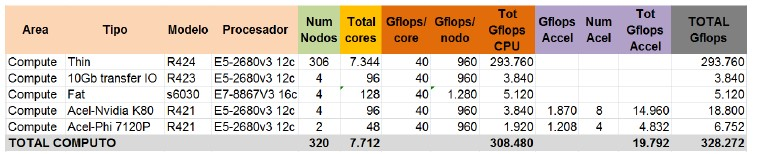
\includegraphics[width=15cm]{figuras/FT2_1.jpg}}
\caption{Arquitectura do \gls{FT2}. Parte 1.}
\medskip
\small
\centerline{Fonte: \url{https://cesga.es/gl/infraestructuras/computacion/FinisTerrae2}}
\label{FT2_1}
\end{figure}

\begin{figure}
\centerline{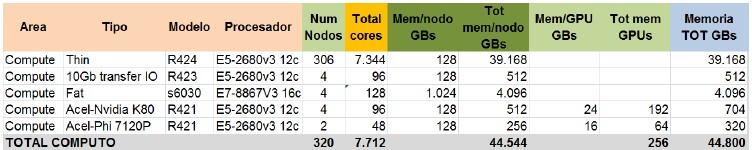
\includegraphics[width=15cm]{figuras/FT2_2.jpg}}
\caption{Arquitectura do \gls{FT2}. Parte 2.}
\medskip
\small
\centerline{Fonte: \url{https://cesga.es/gl/infraestructuras/computacion/FinisTerrae2}}
\label{FT2_2}
\end{figure}

\begin{figure}
\centerline{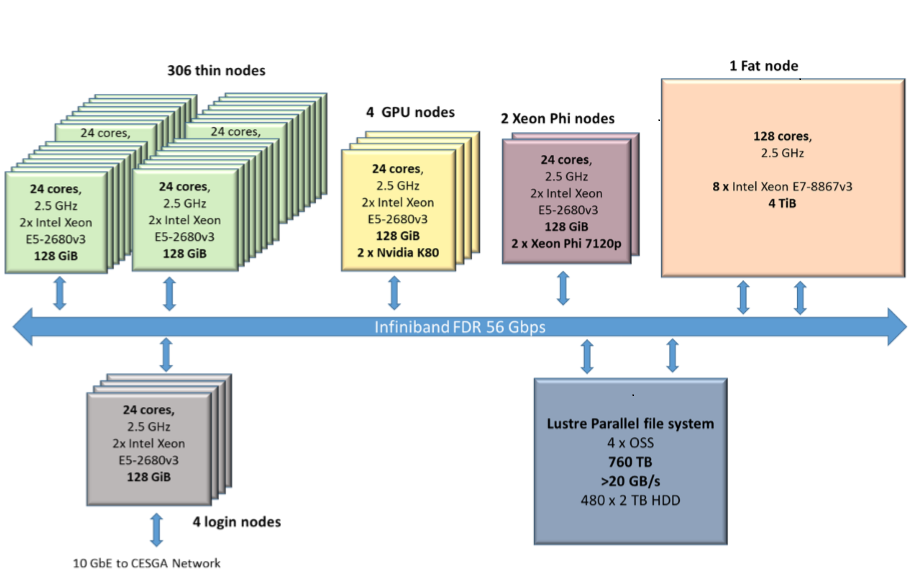
\includegraphics[width=15cm]{figuras/infraFTII.png}}
\caption{Arquitectura do \gls{FT2}. Parte 3.}
\medskip
\small
\centerline{Fonte: \cite{MSO4SC}}
\label{FT2_3}
\end{figure}

\begin{figure}
\centerline{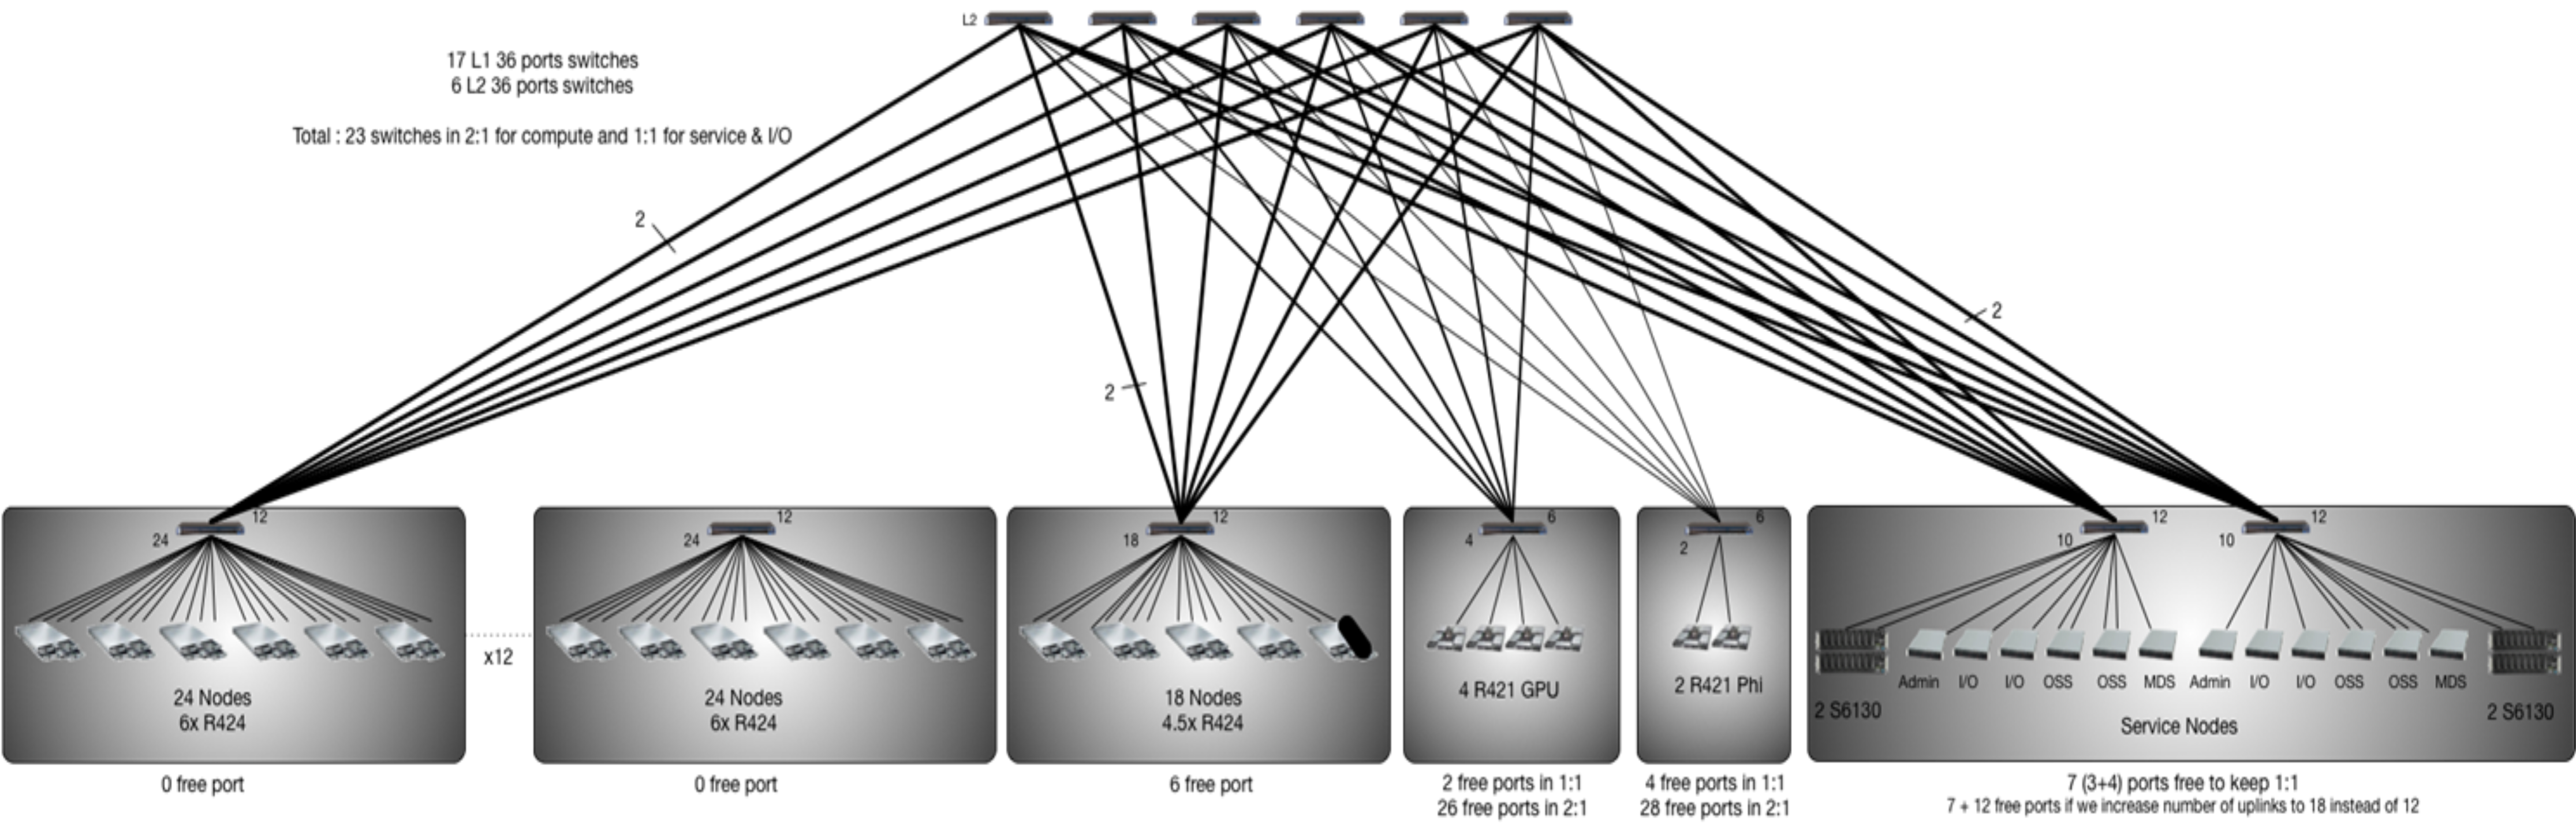
\includegraphics[width=15cm]{figuras/InfiniBand.png}}
\caption{Diagrama da rede InfiniBand do \gls{FT2}}
\medskip
\small
\centerline{Fonte: \url{https://cesga.es/gl/infraestructuras/computacion/FinisTerrae2}}
\label{InfiniBandFigura}
\end{figure}

\section{Contedores e \gls{HPC}}

A emprega de contedores permite a execución de múltiples entornos baixo unha máquina anfitrioa común, o cal supón un mellor aproveitamento do sistema e a posibilidade de establecer separacións máis claras sobre os diferentes procesos. Estas vantaxes tamén son aportadas por outras tecnoloxías de virtualización, como poden ser as máquinas virtuais; no entanto, o uso de contedores supón outra serie de melloras como pode ser a compartición do \textit{kernel} coa máquina anfitrioa, empregando soamente capas lixeiras para o sistema operativo \cite{OS-level-security}. Como resultado, a virtualización a nivel de sistema operativo supón unha perda de rendemento moito menor en comparación con outras tecnoloxías de virtualización, que poden chegar a ser consideradas desprezábeis. Tamén debemos ter en conta que cando traballamos con máquinas virtuais estamos a crear sistemas cuns límites moi definidos (en termos de CPU, memoria e demais recursos), que deben ser restruturados se os queremos ampliar e que moi probabelmente non sexan empregados na súa totalidade, ou ao menos na meirande parte do tempo. Non obstante, a emprega de contedores permite uns límites máis laxos que se adaptan aos recursos dispoñíbeis, contando coa vantaxe de poder establecer uns límites máximos en moitos dos casos, dependendo da tecnoloxía de virtualización.\\

Este achegamento do rendemento a niveis practicamente nativos fai dos contedores unha alternativa moi a ter en conta en entornos de computación de altas prestacións, xunto cos seguintes motivos:

\begin{itemize}
    \item \textbf{Desenvolvemento áxil:} o desenvolvemento tradicional de software en entornos \gls{HPC} presenta algunhas características que o fan moi inflexíbel. O desenvolvemento e integración tradicionais de software baséanse na realización de todos os pasos precisos, como a descarga, configuración, construción, realización de probas e instalación, para ter o software correndo na infraestrutura de produción. Cando traballamos con software científico debemos ter en conta que acostuma ser un software extremadamente complexo dende o punto de vista arquitectónico. Adoita incluír numerosos conceptos e características matemáticas implantados ao longo de varios compoñentes software para prover capas de abstracción a alto nivel. Ditas capas poden estar implantadas directamente no proxecto de software ou integradas a través de librarías de terceiros, polo que o entorno enteiro de software científico supón finalmente unha composición complexa de matrices de dependencias entre diferentes programas e librarías. Todo este proceso pode ser simplificado se empaquetamos todas as librarías e dependencias precisas dentro dun contedor, sobre todo se temos en conta que o proceso de despregamento dun contedor resulta relativamente áxil grazas ao seu pequeno tamaño.
    
    Tamén debe ser tido en conta que certos programas evolucionan moi rápido, empregando últimas tecnoloxías e dependencias difíciles de satisfacer, ao levar esta elevada frecuencia de actualización. Tal tarefa exerce moita presión sobre o equipo de soporte de software de infraestruturas multiusuario como pode ser o \gls{CESGA}.
    
    \item \textbf{Illamento:} o illamento e a integración de todas as matrices de dependencias previamente nomeadas en \textit{clústeres} de \gls{HPC} xestiónanse tradicionalmente mediante módulos de entorno. Por exemplo, Lmod\footnote{\url{https://lmod.readthedocs.io/en/latest/}}, un sistema de módulos baseado en Lua, está a ser empregado no \gls{FT2}. A principal vantaxe destes módulos de entorno é que permiten empregar múltiples versións dun programa ou paquete dende a mesma conta simplemente cargando o ficheiro do módulo axeitado. É posíbel cargar, descargar ou cambiar dinamicamente estes módulos, amais de existir a posibilidade de implantar políticas de acceso e emprega. Polo tanto, podemos concluír que os módulos permiten unha administración de entornos para a execución dunha aplicación nunha versión particular. Non obstante, administrar fluxos complexos de traballo con módulos de entorno pode ser ás veces inalcanzábel e requirir a reinstalación dalgunhas ferramentas coas dependencias compatíbeis. Estes problemas son difíciles de xestionar dende o punto de vista do usuario e o administrador. Así, esta creación de entornos illados para o usuario pode ser simplificada, ou mellorada, mediante a súa substitución ou combinación dos módulos con contedores.
    
    \item \textbf{Integración con entornos \gls{HPC}:} o ecosistema hardware e software dunha infraestrutura de produción de \gls{HPC} é diferente ao ecosistema de desenvolvemento, e xeralmente aparecen moitos problemas inesperados ao integrar e implantar o entorno de software científico, no que están presentes grandes matrices de dependencias. Este feito provoca que integrar todo o entorno de cada un dos proxectos software na infraestrutura de produción adoite ser difícil e requira de moito tempo, xa que o entorno de desenvolvemento debe ser adecuado ao de produción. Por exemplo, se o software vai facer emprega de computación paralela mediante \gls{MPI} sobre InfiniBand, o máis probábel é que haxa que configuralo para que se comunique correctamente con dita rede, provindo os controladores precisos e outros posíbeis cambios. Namentres, un entorno baseado en contedores permitiría ter configuradas todas as dependencias precisas, igualando os entornos de desenvolvemento e produción. Grazas ao xeito de funcionar dos contedores, nos que a virtualización faise simplemente a nivel de sistema operativo, quedando exentas virtualizacións do hardware, podemos facer uso do hardware propio da máquina anfitrioa e así aproveitar características como redes de baixa latencia (InfiniBand) ou incluso procesamento paralelo con unidades de procesamento gráfico (\gls{GPU}s), se o entorno é correctamente configurado no contedor.
\end{itemize}

Os centros de supercomputación ofertan os seus servizos computacionais a unha comunidade científica variada e múltiple, polo que non só deben afrontar o desafío de manter o software actualizado, senón que en moitas ocasións será preciso ter configuradas diferentes versións dun mesmo software, por mor de dependencias entre os mesmos. Esta necesidade pode ser solventada mediante a emprega dos xa nomeados sistemas de módulos ou mediante entornos virtuais. Dende o punto de vista administrativo, as compilacións automáticas e a correcta configuración dun servidor fan posíbel o mantemento destes clústeres \gls{HPC}. Para acadar dita configuración, o habitual é facer uso de xestores de recursos, como pode Slurm, o cal está a ser empregado no \gls{CESGA} e cuxo funcionamento está brevemente explicado na sección \ref{infraestruturaSlurm}. Ditos xestores permiten que os usuarios poidan empregar os recursos ofertados polo centro e tamén aseguran que ditos recursos non se vexan superados debido a unha sobreasignación. \cite{singularityScientificContainers}

\section{Xestor de recursos Slurm}
\label{infraestruturaSlurm}

Posto que no \gls{CESGA} é precisa a execución de numerosos procesos provintes de diferentes usuarios, cómpre contar cun xestor dos recursos físicos presentados na sección \ref{recursosFT2} para poder repartir devanditos recursos dun xeito adecuado, evitando a emprega daqueles que non pertencen a un. Deste xeito, limitando a execución dos procesos a uns recursos concretos, evítase que un determinado programa póidase exceder na emprega dos mesmos e limitar así a execución doutros.\\

Para todo isto, nestes momentos, no centro emprégase o xestor de recursos Slurm, concretamente a versión 14.11.11-Bull.1.7. Trátase dun xestor tolerante a fallas e altamente escalable para clústeres GNU/Linux que permite a programación de traballos. Coma administrador da carga do sistema, Slurm ten tres funcións clave:

\begin{enumerate}
\item Asignar certos recursos de xeito exclusivo aos usuarios que os demanden, durante un tempo determinado, para que poidan desenvolver o seu traballo.
\item Fornecer un marco para iniciar, executar e supervisar o traballo no conxunto de nodos asignados.
\item Arbitrar a disputa polos recursos demandados e administrar unha cola de traballos pendentes.
\end{enumerate}

No referente á súa arquitectura, Slurm ten un administrador centralizado, \textit{slurmctld}, para supervisar os recursos e os traballos. Cada nodo de cómputo posúe un demo \textit{slurmd}, encargado de esperar os traballos, executalos e devolver a súa saída. De cara ao usuario, estes recursos son empregados baixo unha serie de comandos, coma poden ser:

\begin{itemize}
    \item {\it \textbf{srun:}} para iniciar traballos, facendo reserva dos recursos precisos.
    \item {\it \textbf{sbatch:}} para enviar procesos para a súa posterior execución.
    \item {\it \textbf{scancel:}} para cancelar traballos en cola ou en execución.
    \item {\it \textbf{squeue:}} para obter información do estado dos traballos.
\end{itemize}

\begin{figure}
\label{archSingularity}
\centerline{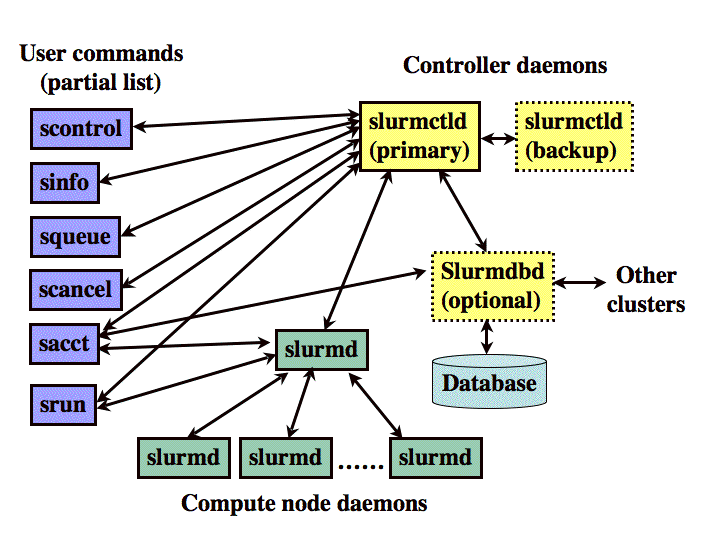
\includegraphics[width=15cm]{figuras/archSingularity.png}}
\caption{Arquitectura de Slurm}
\medskip
\small
\centerline{Fonte: \url{https://slurm.schedmd.com/quickstart.html}}
\end{figure}

A arquitectura do xestor de recursos Slurm pode ser apreciada na figura \ref{archSingularity}. Se o lector desexa ampliar os seus coñecementos acerca do mesmo, pode consultar a documentación oficial\footnote{\url{https://slurm.schedmd.com/}}.

\section{Alternativas: \gls{MV}s fronte a contedores}

A necesidade de crear entornos illados e portábeis non se trata de ningunha novidade. As máquinas virtuais xa introduciron hai tempo esta idea, coa posibilidade de incluír no seu interior todas as dependencias software precisas, librarías, código e datos, para seren executadas en calquera lugar.\\

As \gls{MV}s permiten a creación de entornos completamente illados, facendo segura a outorga de privilexios de superusuario no seu interior aos usuarios. As \gls{MV}s posúen un sistema operativo completo, incluíndo unha propia administración da memoria e a emprega de controladores para dispositivos virtuais. Debido ao uso que fai do hipervisor, este impide que unha \gls{MV} poida executar instrucións que poñan en risco a integridade da máquina anfitrioa \cite{introduccionContainerSecurityDocker}. Non obstante, este illamento tamén engade complexidades adicionais cando tentamos que os entornos contidos no interior das \gls{MV} fagan uso de recursos propios da máquina anfitrioa, como poden ser redes escalábeis como InfiniBand, aceleradores hardware \cite{singularityScientificContainers} ou unidades de procesamento gráfico para computación paralela, recursos amplamente empregados en centros de supercomputación.\\

Coa incorporación de funcións de virtualización lixeiras para o \textit{kernel} de GNU/Linux, por exemplo, coa implantación dos espazos de nomes, foi posíbel implantar unha nova forma de virtualización: a virtualización a nivel de sistema operativo, tamén coñecida como contedores. Este tipo de virtualización presenta a gran vantaxe fronte ás \gls{MV}s que poden compartir unha serie de recursos coa máquina anfitrioa, supondo unha penalización de rendemento moi pequena e en case calquera caso desprezábel. Dito funcionamento fai que os contedores sexan máis lixeiros, rápidos e doados de escalar que as \gls{MV}s, permitindo un funcionamento moito máis flexíbel \cite{introduccionContainerSecurityDocker}. Deste xeito, os contedores permitiron a creación de entornos personalizábeis polo usuario cunha perda de mínima de rendemento, pondo solución ao complexo problema de dependencias software.\\

Podemos concluír que ambos, contedores e \gls{MV}s, provén entornos illados para a execución de aplicacións baixo unha máquina anfitrioa compartida, pero baixo perspectivas técnicas ben distintas. Estas solucións poden ser empregadas de forma independente ou en conxunto, dependendo das necesidades do entorno. Por exemplo, unha boa solución de compromiso entre seguridade e utilidade podería pasar polo despregamento de contedores dentro de \gls{MV}s. Este enfoque aumenta a seguridade ao introducir dúas capas de virtualización, as \gls{MV}s e os contedores, ademais de ofertar os beneficios de despregamento rápido outorgados polos contedores. Polo tanto, pódese acadar un illamento de aplicacións máis sólido combinando a virtualización mediante \gls{MV}s e a contedorización. A figura \ref{CombinacionVirtualizacion} amosa unha representación gráfica de dita implantación. Non obstante, existen certos escenarios que poden non ser bos candidatos para a emprega de \gls{MV}s e nos que no seu canto, o uso de contedores supón unha mellor solución. Por exemplo, aplicacións de rendemento crítico ou aplicacións que fagan uso de hardware especializado no que sexa preciso un acceso directo ao mesmo, supondo neste caso un problema os beneficios do alto illamento dado polas \gls{MV}s. Este é o caso dos centros de supercomputación, como pode ser o \gls{CESGA}, por exemplo, coa execución de aplicacións de procesamento paralelo que fagan uso da \gls{GPU}.

\begin{figure}
\centerline{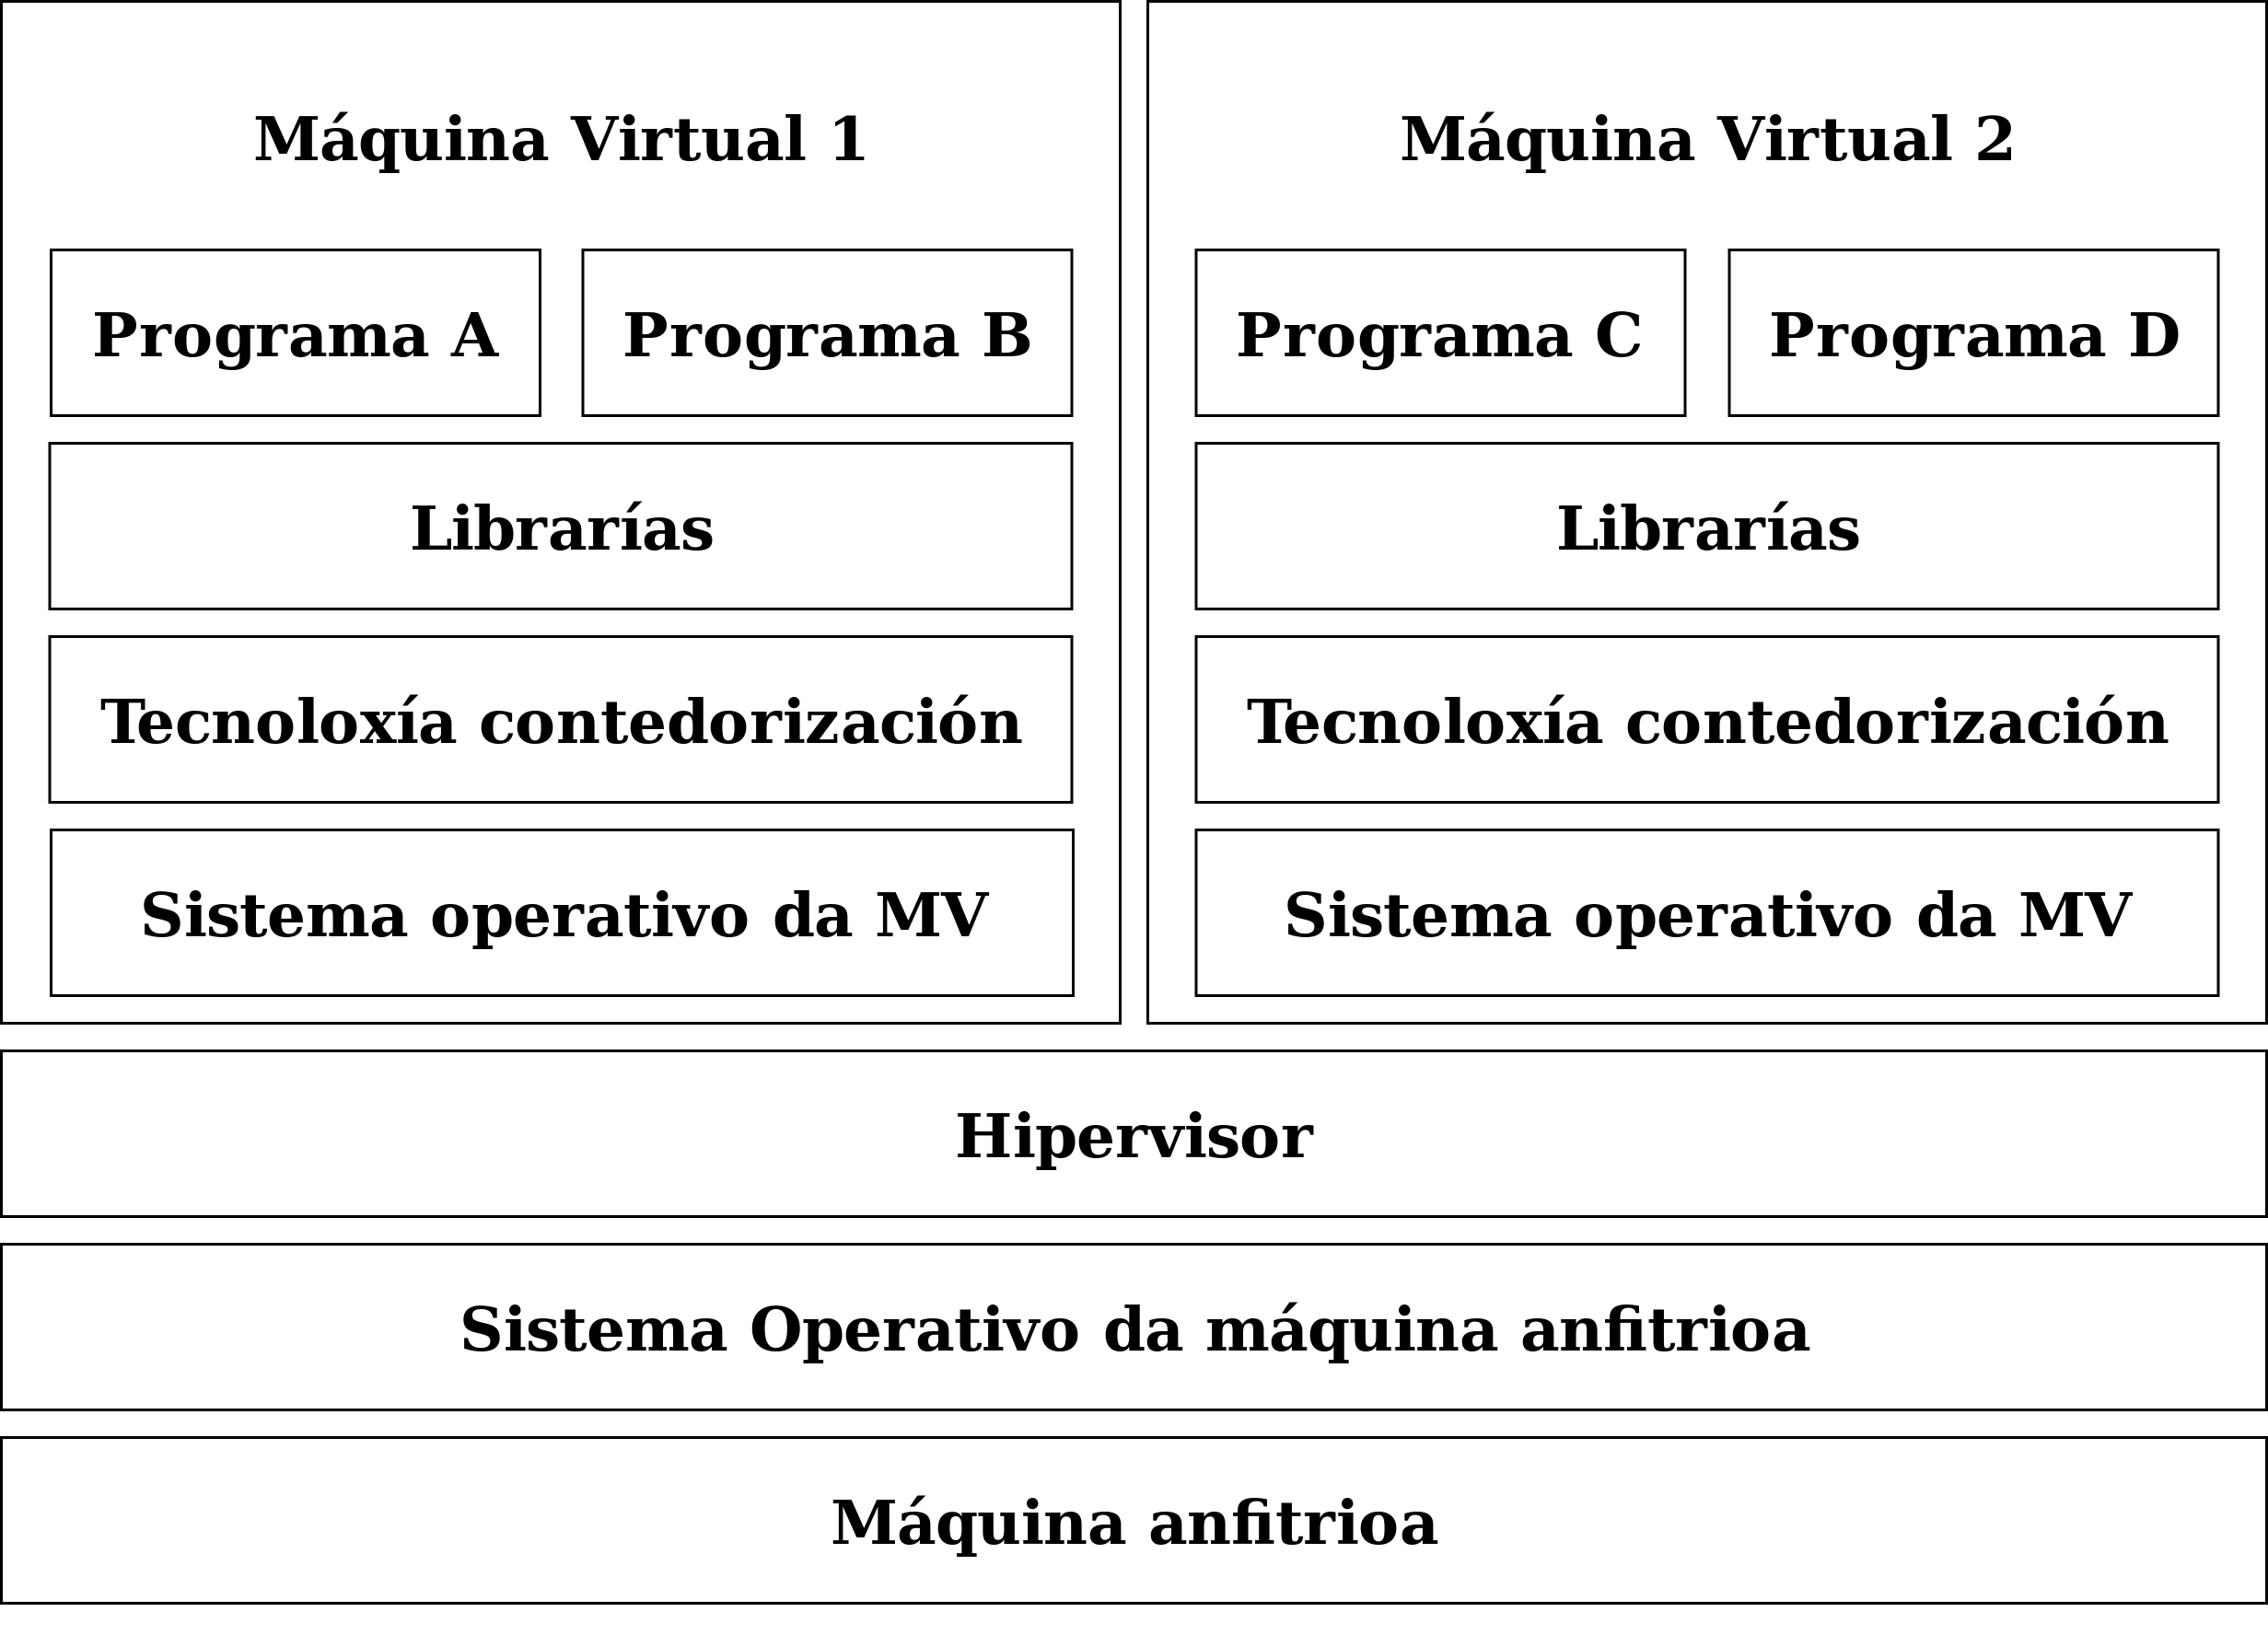
\includegraphics[width=15cm]{figuras/CombinacionVirtualizacion.png}}
\caption{Combinación das tecnoloxías de virtualización}
\label{CombinacionVirtualizacion}
\end{figure}

\section{Computación na nube no \gls{CESGA}}

A computación na nube (ou \textit{Cloud Computing}) é un paradigma que permite ofertar servizos de computación a través dunha rede, habitualmente Internet. O \gls{CESGA} dispón un servizo de computación na nube no cal é posíbel entregar aos usuarios unha infraestrutura de computación virtual e configurábel á medida e requisitos do usuario final: sistema operativo, número de procesadores, memoria, disco e número de nodos son determinados á medida do usuario de forma dinámica. Para a xestión do sistema utilízase o software OpenNebula\footnote{\url{https://opennebula.org/}}. \cite{CloudCESGA}\\

Posto que non todas as probas poderán ser feitas directamente sobre contedores correndo no \gls{FT2}, motivado principalmente pola falta de permisos de execución, farase uso dos servizos de computación na nube para despregar máquinas virtuais sobre as cales poder configurar todos os requirimentos necesarios.

\section{Conclusións}

A diversidade existente na comunidade que fai uso destes recursos de computación de altas prestacións provoca que os centros \gls{HPC} deban manter sistemas estábeis, fiábeis e funcionais, o que moitas veces implica a conserva de sistemas en versións antigas e xa amplamente testadas. No entanto, hoxe en día, a integración continua, as metodoloxías de desenvolvemento áxiles e os lanzamentos continuos (\textit{rolling realeases}) son conceptos cada vez máis empregados no desenvolvemento do software científico. Posuír un software \gls{HPC} mantido ao día neste escenario e seguir a empregar integracións e despregamentos tradicionais, xunto sistemas non actualizados, supón un problema de engarrafamento. Unha das solucións máis flexíbeis e soadas nestes días podería pasar pola emprega de contedores. Polo tanto, podemos dicir que a necesidade á que dan resposta os contedores é ofertar unha maneira simple e eficiente que permita implantar e despregar este complexo software con todas as súas dependencias, sen perder a capacidade computacional dun sistema de \gls{HPC}. Porén, aínda que son moitos os beneficios aportados polos contedores, non debemos esquecer que posúen unha serie de características que fan que a súa seguridade teña que ser estudada con cautela. Ao longo deste documento estudaremos tales características.